\documentclass[11pt,a4paper]{article}
\usepackage[margin=22mm]{geometry}
\usepackage{amsmath,amssymb,booktabs,tikz,enumitem,hyperref}
\usetikzlibrary{arrows.meta,positioning}
\hypersetup{colorlinks=true,urlcolor=blue}
\setlength{\parindent}{0pt}\setlength{\parskip}{7pt}
\newcommand{\question}[2]{\section*{#1: #2}}
\begin{document}
\begin{center}{\Large\bfseries Homework Set 1: AI Introduction}\\[4pt]English worked answers for handwriting\end{center}
\small Original questions: requirements/AI-2026-homeWork-Set-1.pdf, pp.\ 1--3. Due October 10, 2026.\normalsize

\question{Intro1}{What does ``act rationally'' mean?}
To act rationally is to choose the action that is expected to best achieve one's goals, given the available information, possible actions, and consequences. In AI, a rational agent chooses an action that maximizes its expected performance measure or utility:
\[
a^*\in\arg\max_{a}\mathbb{E}[U\mid\text{available information},a].
\]
Rationality describes \emph{how} a decision is made, whereas selfishness describes \emph{whose interests} the goals serve. A selfish person can act rationally by choosing the action with the greatest expected personal benefit. An altruistic person can also act rationally when the objective includes other people's welfare.

For example, a self-interested buyer who compares the prices and quality of several products and chooses the best value is acting rationally. A rational decision need not produce the best actual outcome: uncertainty can make a well-reasoned choice turn out badly. Rationality therefore does not mean omniscience, perfect prediction, or moral goodness.

\question{Intro2}{A task that humans do not do well}
One example is exhaustively searching millions of possible moves in a complex game within a short time. Humans have limited working memory and calculation speed, so they cannot reliably enumerate and compare such a large number of possibilities. They often rely on intuition and may overlook a promising continuation.

A computer can systematically explore many candidate moves, use an evaluation function to estimate their quality, and use search methods to select a strong move. This illustrates that AI can improve technology by using computational abilities that differ from human reasoning. It does not have to imitate the exact way a human thinks.

\newpage
\question{Intro3}{Why did moving to multilayer networks take years?}
\textbf{LLM use.} This answer was developed through the current Codex LLM conversation on October 8, 2026. The question asked was why the XOR limitation mattered, when the important developments occurred, and why adding a hidden layer was not sufficient by itself. The historical dates below were checked against the publisher's book record and the original 1986 paper.

\textbf{The limitation.} XOR has outputs
\[
(0,0)\mapsto0,\quad(0,1)\mapsto1,\quad(1,0)\mapsto1,\quad(1,1)\mapsto0.
\]
The positive and negative examples cannot be separated by one straight line. A perceptron with one trainable layer implements a linear decision boundary, so it cannot represent XOR. Minsky and Papert's \emph{Perceptrons} was published in 1969 [1] and became an important historical milestone in the discussion of perceptron limitations.

\textbf{What a hidden layer changes.} Nonlinear hidden units can form intermediate features, which an output unit combines to represent a nonlinear decision boundary. For example, let $H(z)=1$ for $z\geq0$ and $0$ otherwise. The following small network computes XOR:
\[
z_1=H(x_1+x_2-0.5),\qquad z_2=H(x_1+x_2-1.5),
\qquad y=H(z_1-2z_2-0.5).
\]
Here $z_1$ computes OR and $z_2$ computes AND. For the four inputs, $(z_1,z_2)$ equals $(0,0),(1,0),(1,0),(1,1)$, giving $y=0,1,1,0$.

\begin{center}
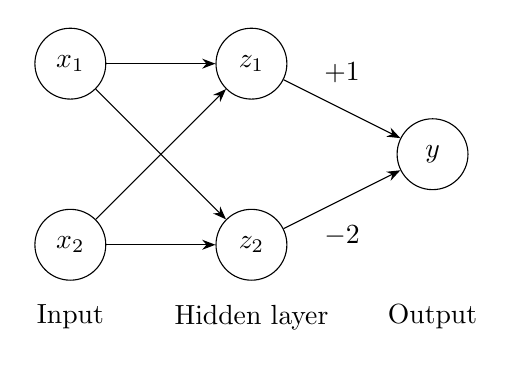
\begin{tikzpicture}[>=Stealth,every node/.style={draw,circle,minimum size=9mm},x=2.3cm,y=1.15cm]
\node (x1) at (0,1) {$x_1$};\node (x2) at (0,-1) {$x_2$};
\node (z1) at (1,1) {$z_1$};\node (z2) at (1,-1) {$z_2$};\node (y) at (2,0) {$y$};
\foreach \a in {x1,x2}\foreach \b in {z1,z2}\draw[->] (\a)--(\b);
\draw[->] (z1)--node[draw=none,above] {$+1$}(y);
\draw[->] (z2)--node[draw=none,below] {$-2$}(y);
\node[draw=none,rectangle] at (0,-1.8) {Input};
\node[draw=none,rectangle] at (1,-1.8) {Hidden layer};
\node[draw=none,rectangle] at (2,-1.8) {Output};
\end{tikzpicture}
\end{center}
\textbf{Why this was not merely ``add one layer.''} Constructing weights manually for XOR is different from learning the weights of a general multilayer network. Hidden units have no directly supplied target outputs, so a learning method must determine how each hidden weight contributed to the final error. Nonlinear differentiable activations, the chain rule, gradient-based optimization, and error back-propagation make this credit assignment possible. The hard-threshold example above demonstrates representation; practical back-propagation uses differentiable units instead.

\newpage
\textbf{Historical interval.} Rumelhart, Hinton, and Williams published \emph{Learning representations by back-propagating errors} in 1986 [2]. It explained how output errors could be propagated through hidden layers to adjust weights and learn useful internal representations. This was a major milestone in popularizing multilayer learning, not the first-ever invention of multilayer networks or all forms of back-propagation.

Using the homework's approximate 1970 starting point and the 1986 milestone gives
\[
1986-1970=\boxed{16\text{ years}}.
\]
Using the actual 1969 publication of \emph{Perceptrons} gives 17 years. Thus the intended historical interval is approximately sixteen to seventeen years, depending on the chosen starting point.

The statement that ``neural networks were dead'' around 1970 is a simplified description of a decline in interest. It should not be read as a proof that all neural networks were incapable of XOR or that no relevant research occurred during that period. The key distinction is between \emph{representing} XOR and \emph{learning} useful hidden representations reliably.

\section*{Sources for Intro3}
\begin{enumerate}[label={[\arabic*]}]
\item Marvin Minsky and Seymour A. Papert, \emph{Perceptrons: An Introduction to Computational Geometry}, MIT Press, 1969. Publisher record: \url{https://mitpress.mit.edu/9780262130431/perceptrons/}.
\item David E. Rumelhart, Geoffrey E. Hinton, and Ronald J. Williams, ``Learning representations by back-propagating errors,'' \emph{Nature} 323, 533--536 (1986). DOI: \href{https://doi.org/10.1038/323533a0}{10.1038/323533a0}. Author-hosted original: \url{https://www.cs.toronto.edu/~hinton/absps/naturebp.pdf}.
\end{enumerate}
\end{document}
